% ---------------------------------------------------------------------------
% fig:teaser -- the three challenges of the introduction, before and after.
% Columns = the three challenges; top band = existing practice (muted grey),
% bottom band = MWM (white ground, full colour).  Same slots, different
% outcome: each column's cross and tick share one marker x, and the band-wide
% idea + result sit in a footer so every down-arrow lands on its own column.
% MWM band rows: labels (base 2.96) | vision (2.40) | EEG (1.60) | tags | ticks.
% ---------------------------------------------------------------------------
\definecolor{tztbrick}{HTML}{9A5A50}   % limitation marker (kept apart from latred)
\definecolor{tztgreen}{HTML}{3F8B4E}   % advantage marker (kept apart from vizteal)
% verdict markers, centred on a coordinate #1 = (x,y)
\newcommand{\tztno}[1]{%
  \draw[tztbrick, line width=0.5pt] #1 circle (0.125);
  \draw[tztbrick, line width=0.95pt, line cap=round]
    ($#1+(-0.052,-0.052)$) -- ++(0.104,0.104)
    ($#1+(-0.052, 0.052)$) -- ++(0.104,-0.104);}
\newcommand{\tztok}[1]{%
  \fill[tztgreen] #1 circle (0.165);
  \node[inner sep=0pt, font=\scriptsize, text=white] at ($#1+(0,0.005)$)
    {$\checkmark$};}
% square patch grid centred on (0,0): #1 = n, #2 = cell, #3 = fill, #4 = stroke
\newcommand{\tztgrid}[4]{%
  \pgfmathsetmacro{\gh}{#1*#2/2}
  \foreach \gi in {1,...,#1}{\foreach \gj in {1,...,#1}{
     \fill[#3, draw=#4, line width=0.25pt]
       ({(\gi-1)*#2-\gh},{\gh-(\gj-1)*#2}) rectangle ({\gi*#2-\gh},{\gh-\gj*#2});}}}
% bilateral / lateral feature stack centred on (0,0); #1 = +1 (as recorded)
% or -1 (flipped): only the lateral half turns round (as in the flip figure, panel e)
\newcommand{\tztstack}[1]{%
  \draw[fill=bilight,  draw=bislate, line width=0.6pt] (-0.20,0) rectangle (0.20,0.22);
  \draw[fill=latlight, draw=latred,  line width=0.6pt] (-0.20,-0.22) rectangle (0.20,0);
  \draw[-{Stealth[length=1.4mm,width=1.2mm]}, latred, line width=0.7pt]
    ({-0.13*#1},-0.11) -- ({0.13*#1},-0.11);}

% a hand seen from above, drawn in the muted ink of the "existing" band
\newcommand{\tzthand}{%
  \draw[fill=white, draw=inkgray!60, line width=0.5pt, rounded corners=0.9pt]
    (-0.085,-0.105) rectangle (0.085,0.045);
  \foreach \fx/\fl in {-0.064/0.12, -0.021/0.145, 0.022/0.135, 0.064/0.105}{
    \draw[fill=white, draw=inkgray!60, line width=0.5pt, rounded corners=0.8pt]
      ({\fx-0.018},0.035) rectangle ({\fx+0.018},{0.035+\fl});}
  \draw[fill=white, draw=inkgray!60, line width=0.5pt, rounded corners=0.8pt, rotate around={-38:(0.085,-0.02)}]
    (0.067,-0.03) rectangle (0.103,0.085);}

\begin{tikzpicture}[x=1cm,y=1cm]

\tikzset{
  colhead/.style ={font=\small\bfseries, text=inkgray, inner sep=1pt},
  rowlab/.style  ={font=\scriptsize\bfseries, rotate=90, inner sep=1pt},
  fam/.style     ={font=\scriptsize\itshape, text=inkgray!78, inner sep=1pt},
  capE/.style    ={font=\scriptsize, text=inkgray!80, inner sep=1.5pt, anchor=west},
  capM/.style    ={font=\scriptsize, text=inkgray, inner sep=1.5pt, anchor=west},
  mtag/.style    ={tag},
  etag/.style    ={tag, text=eegblue},
  mflow/.style   ={flow, draw=inkgray!48, line width=0.75pt},
  shot/.style    ={inner sep=0pt, draw=inkgray!45, line width=0.6pt},
  chip/.style    ={draw=inkgray!55, fill=white, line width=0.6pt, rounded corners=1.2pt,
                   font=\scriptsize\bfseries, text=inkgray!75, inner sep=0pt,
                   minimum width=0.36cm, minimum height=0.30cm},
  dot/.style     ={circle, inner sep=0pt, minimum size=3.2pt},
  mlab/.style    ={lbl, font=\footnotesize, anchor=base, inner sep=0pt},
  band/.style    ={-{Stealth[length=1.8mm,width=2.1mm]}, line width=1.1pt, inkgray!55},
  % short hops keep a visible shaft with a smaller tip
  hop/.style     ={-{Stealth[length=1.4mm,width=1.3mm]}},
}

% ============================ bands ======================================
% frames are inset by half their stroke so the body stays within 13.60 cm
% existing practice: a quiet grey band with a light tab
\begin{scope}
  \clip[rounded corners=3pt] (0.011,3.84) rectangle (13.589,5.84);
  \fill[softgray] (0,3.84) rectangle (13.60,5.84);
  \fill[inkgray!22] (0,3.84) rectangle (0.46,5.84);
\end{scope}
\draw[inkgray!25, line width=0.6pt, rounded corners=3pt] (0.011,3.84) rectangle (13.589,5.84);
\node[rowlab, text=inkgray!85] at (0.23,4.84) {Existing};
\foreach \x in {4.70,9.36}{\draw[white, line width=1.4pt] (\x,3.99) -- (\x,5.69);}

% MWM: white ground, dark neutral frame (gold stays reserved for a_t)
\begin{scope}
  \clip[rounded corners=3pt] (0.016,0.44) rectangle (13.584,3.40);
  \fill[white] (0,0.44) rectangle (13.60,3.40);
  \fill[inkgray!85] (0,0.44) rectangle (0.46,3.40);
\end{scope}
\draw[inkgray!70, line width=0.9pt, rounded corners=3pt] (0.016,0.44) rectangle (13.584,3.40);
\node[rowlab, text=white] at (0.23,1.92) {\method{} (ours)};
\draw[inkgray!15, line width=0.6pt] (9.36,0.62) -- (9.36,3.25);

% column headers: the three challenges
\node[colhead] at (2.58,6.12)  {(1) Labels \& data};
\node[colhead] at (7.03,6.12)  {(2) Pretraining target};
\node[colhead] at (11.48,6.12) {(3) Lateralization};


% existing -> MWM, per column
\foreach \x in {2.58,7.03,11.48}{\draw[band] (\x,3.78) -- (\x,3.44);}

% verdicts: one marker x per column, both captions start at the same x
\foreach \mx/\te/\tm in {
    0.81/{costly trials, coarse labels}/{no manual annotations, full observation},
    5.46/{target: the EEG itself}/{target: behavior's consequences},
    9.72/{no explicit lateral modelling}/{explicit lateral modelling}}{
  \node[capE] at ({\mx+0.20},4.10) {\te};
  \node[capM] at ({\mx+0.20},0.80) {\tm};
  \tztno{(\mx,4.10)}
  \tztok{(\mx,0.80)}}

% ================= (1) existing: cue trials -> {L, R} ====================
\begin{scope}[shift={(2.83,4.94)}]
  \foreach \d in {0.14,0.07}{
    \draw[fill=white, draw=inkgray!28, line width=0.5pt, rounded corners=1pt]
      ({-1.93+\d},{-0.06+\d}) rectangle ({-1.11+\d},{0.48+\d});}
  \draw[fill=white, draw=inkgray!55, line width=0.6pt, rounded corners=1pt]
    (-1.93,-0.06) rectangle (-1.11,0.48);
  \draw[-{Stealth[length=1.5mm,width=1.9mm]}, line width=1.5pt, inkgray!60]
    (-1.29,0.21) -- (-1.76,0.21);
  \draw[inkgray!55, line width=0.6pt] (-1.52,-0.06) -- (-1.52,-0.16)
    (-1.68,-0.16) -- (-1.36,-0.16);
  \node[mtag] at (-1.45,-0.48) {cue trials};
  % two different left-hand movements -- a slow reach and a fast grasp --
  % end up as the same class in a two-word vocabulary
  \begin{scope}[shift={(-0.70,0.50)}] \tzthand \end{scope}
  \begin{scope}[shift={(-0.70,-0.02)}] \tzthand \end{scope}
  \draw[inkgray!48, line width=0.75pt] (-0.54,0.50) to[out=8, in=178] (0.52,0.30);
  \draw[inkgray!48, line width=0.75pt] plot[domain=0:1, samples=70, smooth]
    ({-0.54+1.06*\x}, {-0.02+0.32*\x + 0.10*sin(1440*\x)*(1-\x)});
  \node[tag, text=inkgray!60, anchor=south] at (0.06,0.54) {slow reach};
  \node[tag, text=inkgray!60, anchor=north] at (-0.02,-0.16) {fast grasp};
  \node[draw=inkgray!60, fill=white, line width=0.6pt, rounded corners=1.2pt,
        font=\scriptsize\bfseries, text=inkgray!80, inner xsep=2.5pt, inner ysep=1.5pt]
        (cL) at (1.07,0.30) {left hand};
  \node[draw=inkgray!25, fill=white, line width=0.5pt, rounded corners=1.2pt,
        font=\scriptsize, text=inkgray!35, inner xsep=2.5pt, inner ysep=1.5pt]
        at (1.07,-0.08) {right hand};
  \draw[mflow, -{Stealth[length=1.7mm,width=1.5mm]}] (0.48,0.30) -- (cL.west);
\end{scope}

% ================= (2) existing: clinical EEG, EEG -> EEG ================
\begin{scope}[shift={(7.155,4.70)}]
  % clinical corpus
  \fill[white] (-1.63,0.52) -- (-1.63,0.10) arc (180:360:0.22 and 0.07) -- (-1.19,0.52) -- cycle;
  \draw[inkgray!50, line width=0.6pt, fill=white] (-1.41,0.52) ellipse (0.22 and 0.07);
  \draw[inkgray!50, line width=0.6pt] (-1.63,0.52) -- (-1.63,0.10)
    arc (180:360:0.22 and 0.07) -- (-1.19,0.52);
  \draw[inkgray!55, line width=1.3pt] (-1.41,0.21) -- (-1.41,0.41)
    (-1.51,0.31) -- (-1.31,0.31);
  \node[mtag] at (-1.41,-0.24) {clinical};
  \draw[mflow] (-1.13,0.24) -- (-0.87,0.24);
  % EEG with masked patches
  \begin{scope}[shift={(-0.80,0.44)}] \eegtrace{1.20}{0.54}{3}{inkgray!55} \end{scope}
  \foreach \xa/\ya in {-0.55/0.36, 0.02/0.18, -0.70/0.00}{
    \draw[fill=inkgray!28, draw=inkgray!45, line width=0.4pt, rounded corners=0.8pt]
      (\xa,\ya) rectangle ({\xa+0.28},{\ya+0.16});}
  \draw[mflow] (0.46,0.24) -- (0.72,0.24);
  % encoder
  \draw[fill=white, draw=inkgray!55, line width=0.6pt, rounded corners=1pt]
    (0.78,0.02) -- (0.78,0.46) -- (1.38,0.36) -- (1.38,0.12) -- cycle;
  \node[font=\scriptsize\itshape, text=inkgray!70, inner sep=0pt] at (1.05,0.24) {enc.};
  % ... whose target is EEG again
  \draw[ghost, draw=inkgray!55, rounded corners=3pt]
    (1.08,0.43) -- (1.08,0.82) -- (-0.41,0.82) -- (-0.41,0.56);
  \node[mtag] at (0.30,-0.24) {masked EEG $\rightarrow$ EEG};
\end{scope}

% ================= (1)+(2) MWM: one mechanism answers both ================
% High level on purpose -- the architecture is Figure 2's job. Read as the
% world-model equation  state + action -> next state,  with EEG as the action.
% The two ticks below stay under their own columns: one idea, two outcomes.
\node[font=\footnotesize\itshape, text=inkgray, inner sep=1pt] at (4.91,3.10)
  {EEG as the \textcolor{actgold!65!black}{\bfseries latent action} of a world model};

\node[shot] (cur) at (2.05,2.10)
  {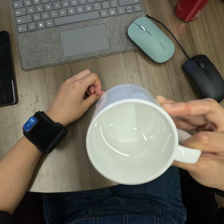
\includegraphics[width=0.82cm, trim=54 34 0 20, clip]{ego_anchor}};
\node[mtag, anchor=north] at (2.05,1.46) {current state};

\node[font=\large, text=inkgray!65, inner sep=0pt] at (3.00,2.10) {$+$};

% the EEG recorded up to the current frame, framed in the action colour
\fill[eeglight, draw=actgold!85!black, line width=0.8pt, rounded corners=2pt]
  (3.40,1.79) rectangle (4.90,2.41);
\begin{scope}
  \clip (3.40,1.79) rectangle (4.90,2.41);
  \begin{scope}[shift={(3.40,2.33)}] \eegtrace{1.50}{0.54}{4}{eegblue} \end{scope}
\end{scope}
\node[mtag, anchor=north, align=center, text=actgold!65!black] at (4.15,1.46)
  {EEG up to now\\[-1pt]= latent action};

% the world model turns state + action into the next state
\draw[-{Stealth[length=2.4mm,width=2.0mm]}, line width=1.4pt, draw=vizteal]
  (5.12,2.10) -- (6.82,2.10);
\node[mtag, anchor=south, text=vizteal!80!black] at (5.97,2.20) {world model};
\node[mtag, anchor=north, text=vizteal!80!black] at (5.97,2.00) {predicts};

\node[shot] (fut) at (7.62,2.10)
  {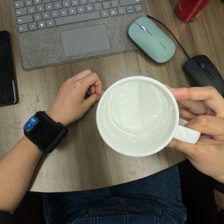
\includegraphics[width=0.82cm, trim=54 34 0 20, clip]{ego_target}};
\node[mtag, anchor=north] at (7.62,1.46) {next state};

% ================= (3) existing: both sides mixed into one feature =======
\begin{scope}[shift={(11.65,5.09)}]
  \begin{scope}[shift={(-0.62,0)}]
    % a muted scalp (the method figures' \headtop is drawn in full ink)
    \draw[fill=white, draw=inkgray!55, line width=0.6pt] (0,0) circle (0.40);
    \draw[inkgray!55, line width=0.6pt] (100:0.40) -- (0,0.487) -- (80:0.40);
    \draw[inkgray!35, line width=0.5pt, dash pattern=on 1.2pt off 1.2pt] (0,-0.40) -- (0,0.40);
    % channel attention links left and right electrodes across the midline
    \foreach \x/\y in {0.21/0.20, 0.28/0.0, 0.21/-0.20}{
      \draw[inkgray!48, line width=0.55pt] (-\x,\y) to[bend left=20] (\x,\y);}
    \foreach \x/\y in {0.21/0.20, 0.28/0.0, 0.21/-0.20}{
      \fill[inkgray!60] (-\x,\y) circle (0.045);
      \fill[inkgray!60] (\x,\y) circle (0.045);}
  \end{scope}
  % hemisphere markers, then one undivided feature that holds both
  \node[font=\scriptsize\bfseries, text=inkgray!70, anchor=east, inner sep=1pt] at (-1.06,0) {L};
  \node[font=\scriptsize\bfseries, text=inkgray!70, anchor=west, inner sep=1pt] at (-0.18,0) {R};
  \draw[mflow] (0.02,0) -- (0.30,0);
  \draw[fill=inkgray!22, draw=inkgray!50, line width=0.6pt] (0.36,-0.22) rectangle (0.76,0.22);
  \node[font=\tiny\bfseries, text=inkgray!75, inner sep=0pt] at (0.56,0) {L+R};
  \node[mtag] at (-0.18,-0.63) {fused into one feature};
\end{scope}

% ================= (3) MWM: paired flip, only H^lat is swapped ===========
% The recorded frame and its mirror image sit above their EEG features:
% flipping the video pairs with keeping H^bi and swapping only H^lat.
% (the mirrored frame uses the mirrored crop, so it is an exact mirror image)
\node[shot] (fA) at (10.30,2.40)
  {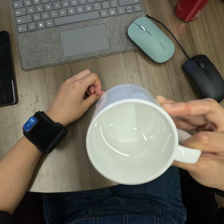
\includegraphics[width=0.82cm, trim=54 34 0 20, clip]{ego_anchor}};
\node[shot] (fB) at (12.64,2.40)
  {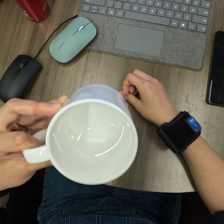
\includegraphics[width=0.82cm, trim=0 34 54 20, clip]{ego_anchor_flip}};
\draw[flow, hop, draw=inkgray!70, line width=0.8pt]
  ([xshift=0.08cm]fA.east) -- ([xshift=-0.08cm]fB.west);
\node[mtag, anchor=base] at (11.47,2.58) {paired flip};
\node[mtag, anchor=base] at (10.30,2.98) {as recorded};
\node[mtag, anchor=base] at (12.64,2.98) {mirrored};
\begin{scope}[shift={(10.30,1.60)}] \tztstack{1} \end{scope}
\begin{scope}[shift={(12.64,1.60)}] \tztstack{-1} \end{scope}
\node[etag, anchor=east] at (10.05,1.60) {EEG};
\node[etag, anchor=west] at (12.89,1.60) {EEG};
% H^bi carried over unchanged, H^lat swapped across hemispheres
\draw[hop, draw=bislate, line width=0.75pt] (10.56,1.71) -- (12.38,1.71);
\draw[hop, draw=latred,  line width=0.75pt] (10.56,1.49) -- (12.38,1.49);
\node[lbl, anchor=base, text=bislate, inner sep=0pt] at (11.47,1.89)
  {{\footnotesize$\mathbf{H}^{\mathrm{bi}}$} kept};
\node[lbl, anchor=base, text=latred, inner sep=0pt] at (11.47,1.105)
  {{\footnotesize$\mathbf{H}^{\mathrm{lat}}$} swapped};

\end{tikzpicture}
